%!TEX root = ../../thesis_main.tex
% The line above allows you to build the main thesis file from this file if you run latexmk.
% This is an example chapter file.
% The \chapter command is in thesis_main.tex so just include text and sections/subsections in this file.

\section{Example section}

This is some introductory text with an example reference to \cref{fig:example} below.
A paper \cite{articlecitekey} or book \cite{strunk1999elements} my be cited like this.
\cref{tab:example} is an example of a table.
You may also like to use acronyms like \gls{tfa} or \gls{aa}.
All these references will hyperlink to the correct place in the document

\begin{figure}[h]
\centering
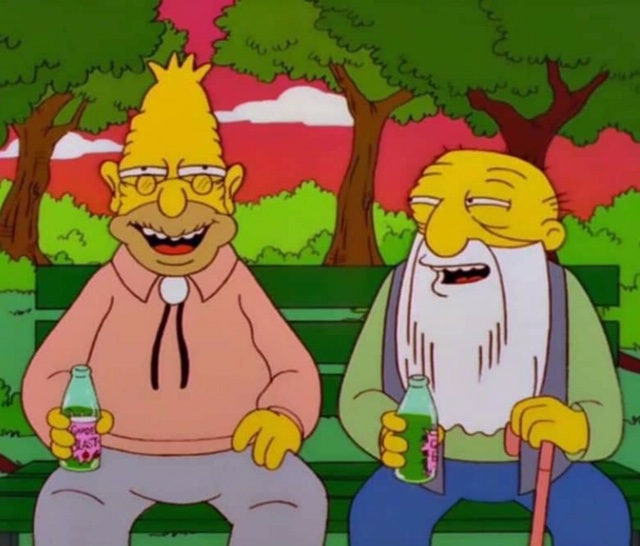
\includegraphics[width=0.5\textwidth]{chapters/chapter_1/figures/example_image.jpg}
\caption{Example of a figure}
\label{fig:example}
\end{figure}

\begin{table}[htb]
\centering
\caption{Example table caption}
\begin{tabular}{c c c c} 
 \hline
 Column 1 & Column 2 & Column 3 & Column 4 \\ 
 \hline\hline
 1 & 6 & 87837 & 787 \\ 
 2 & 7 & 78 & 5415 \\
 3 & 545 & 778 & 7507 \\
 4 & 545 & 18744 & 7560 \\
 5 & 88 & 788 & 6344 \\ 
 \hline
\end{tabular}
\label{tab:example}
\end{table}

\subsection{Example subsection}

Some more text would go here .......
 
And you might want to add a numbered equation like the one below, which can also be referenced in the text as \cref{eq:example}.
\begin{equation} \label{eq:example}
E=mc^2
\end{equation}